\subsubsection{Màn hình 2}
\textbf{Mô tả:} Xem thông tin của phòng ban cùng với thông tin của nhân viên vận hành phòng ban đó. Có tính năng lọc các phòng ban theo số lượng nhân viên tối thiểu. Có tính năng sắp xếp các phòng ban theo thứ tự giảm dần tổng số ngày có mặt của các nhân viên thuộc phòng ban đó.

Màn hình hiển thị thông tin phòng ban, cùng với các nút chức năng
\begin{figure}[H]
    \centering
    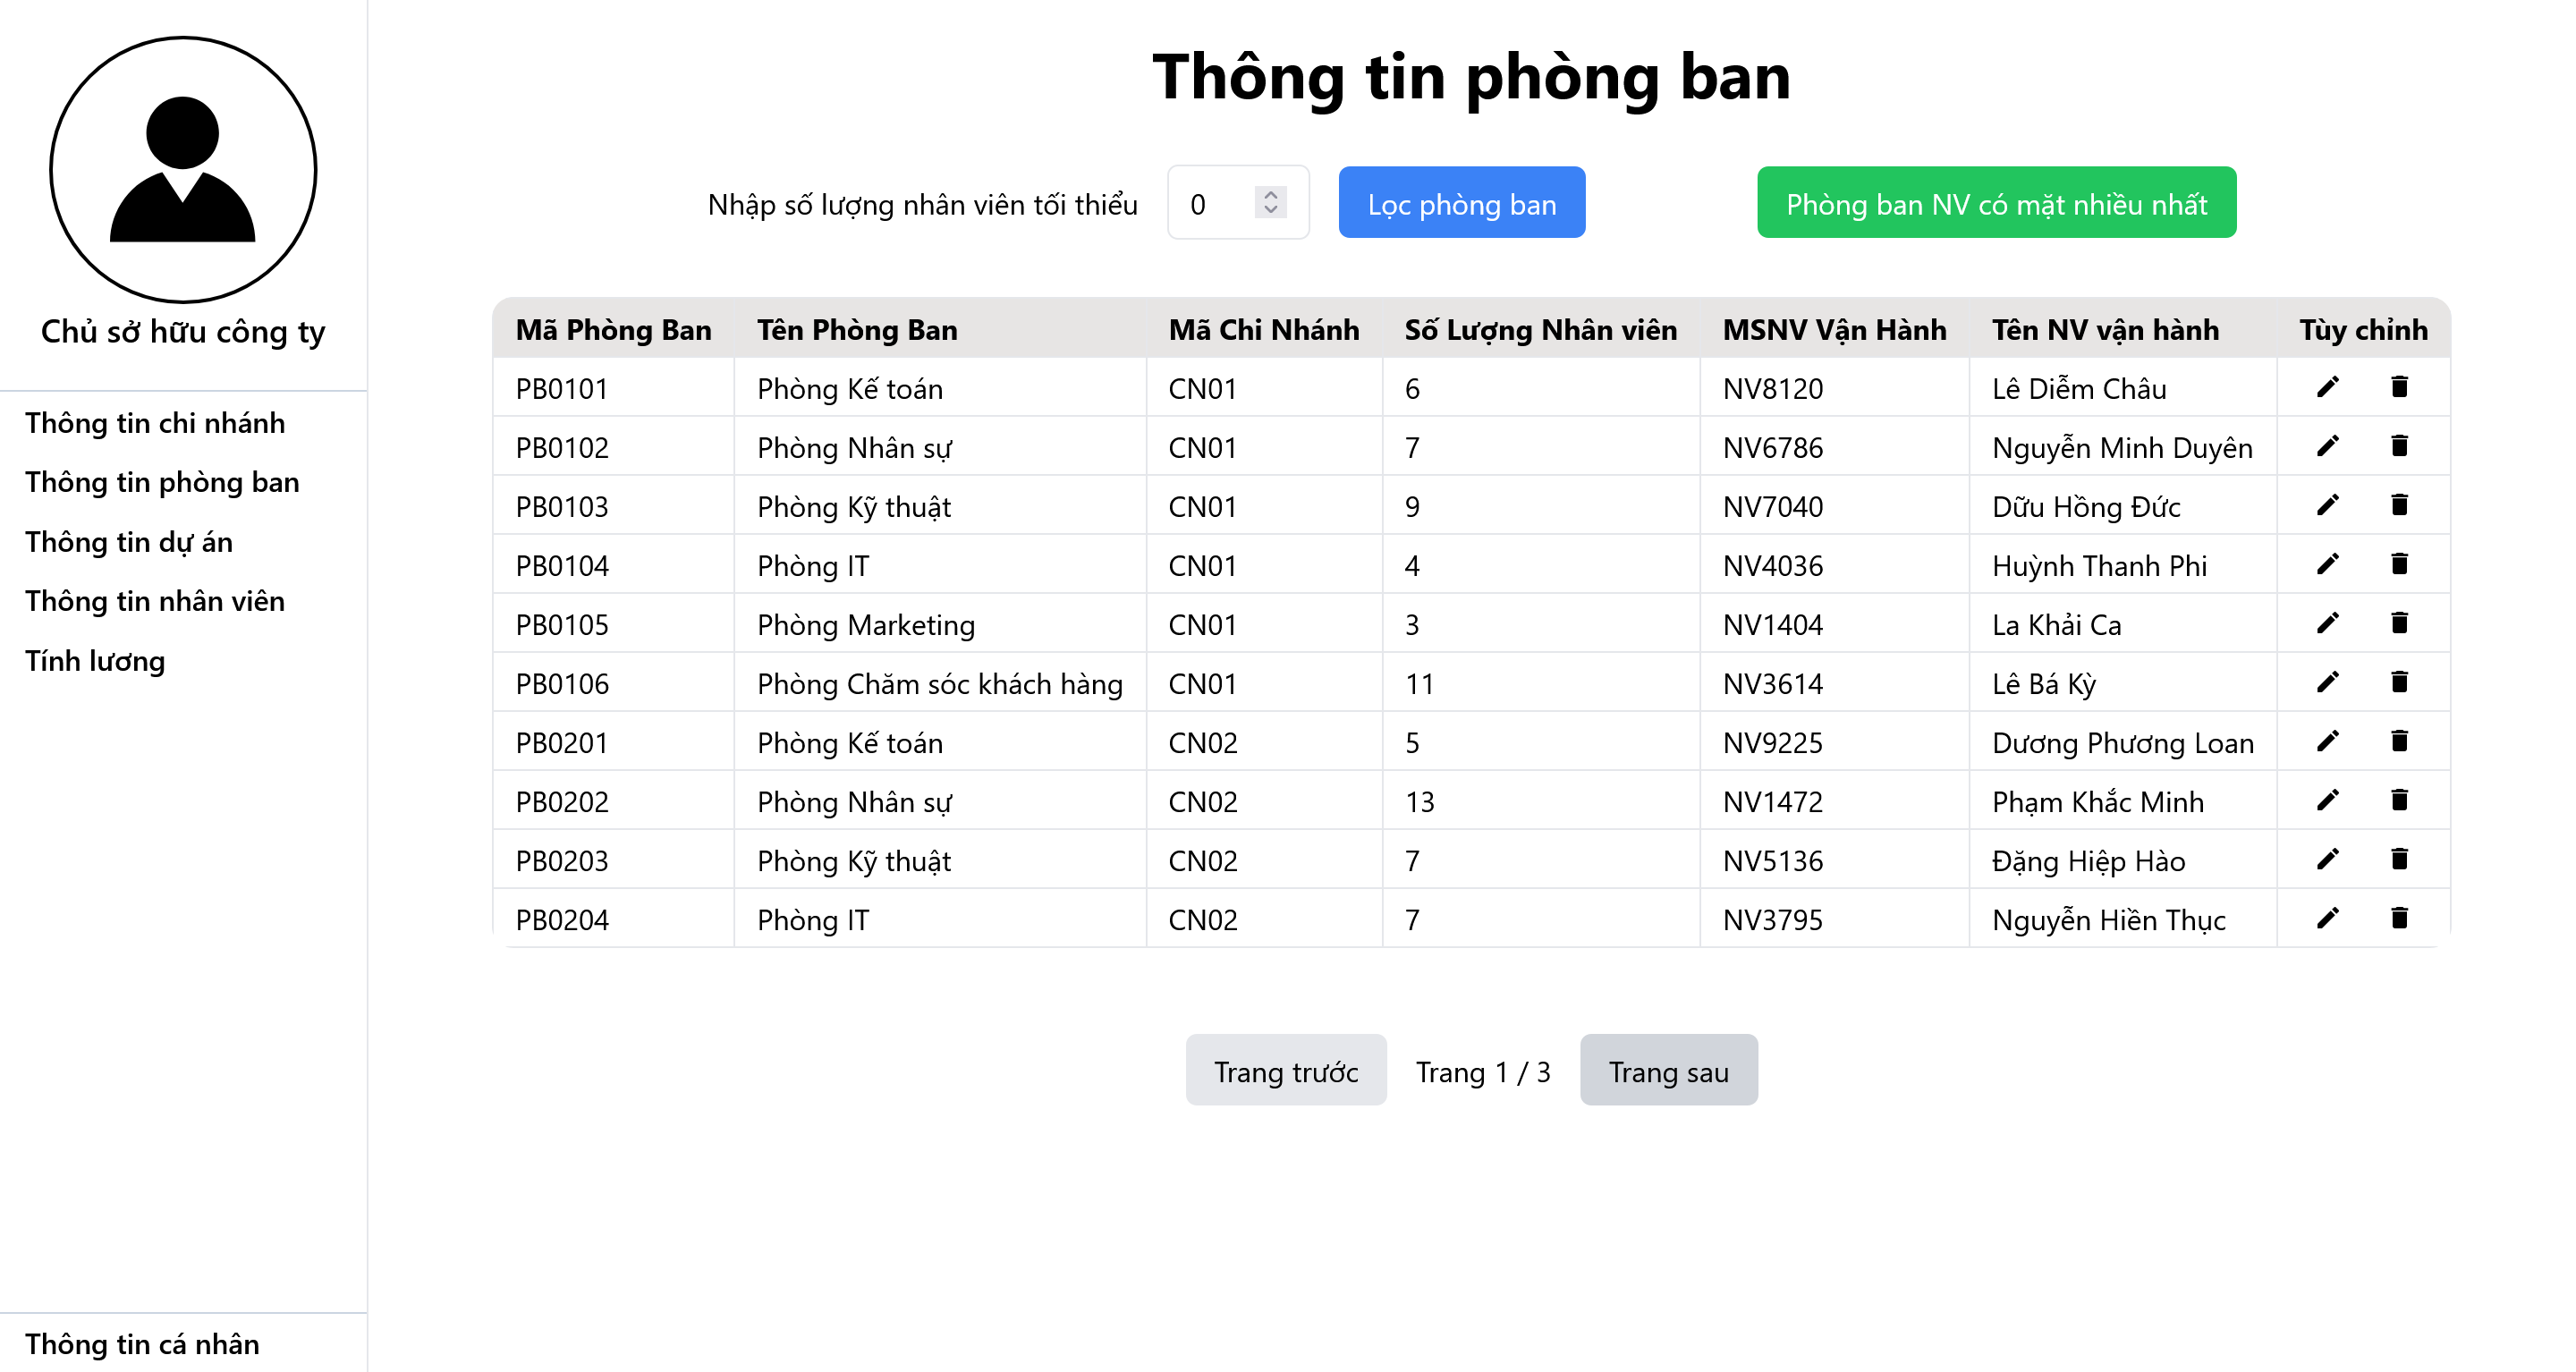
\includegraphics[width=1\linewidth]{content/images/ManHinh_2_a.png}
    \caption{Hiển thị thông tin bảng PhongBan, cùng với các nút chức năng}
    \label{fig:ManHinh_2_a}
\end{figure}

Để sử dụng tính năng lọc các phòng ban theo số lượng nhân viên tối thiểu, người dùng tiến hành nhập số lượng tối thiểu và click vào nút 'Lọc phòng ban'. Màn hình sẽ hiển thị thông tin các phòng ban thỏa mãn tiêu chí đó. Người dùng có thể quay lại xem thông tin phòng ban bằng cách nhấn vào nút 'Tắt lọc'.
\begin{figure}[H]
    \centering
    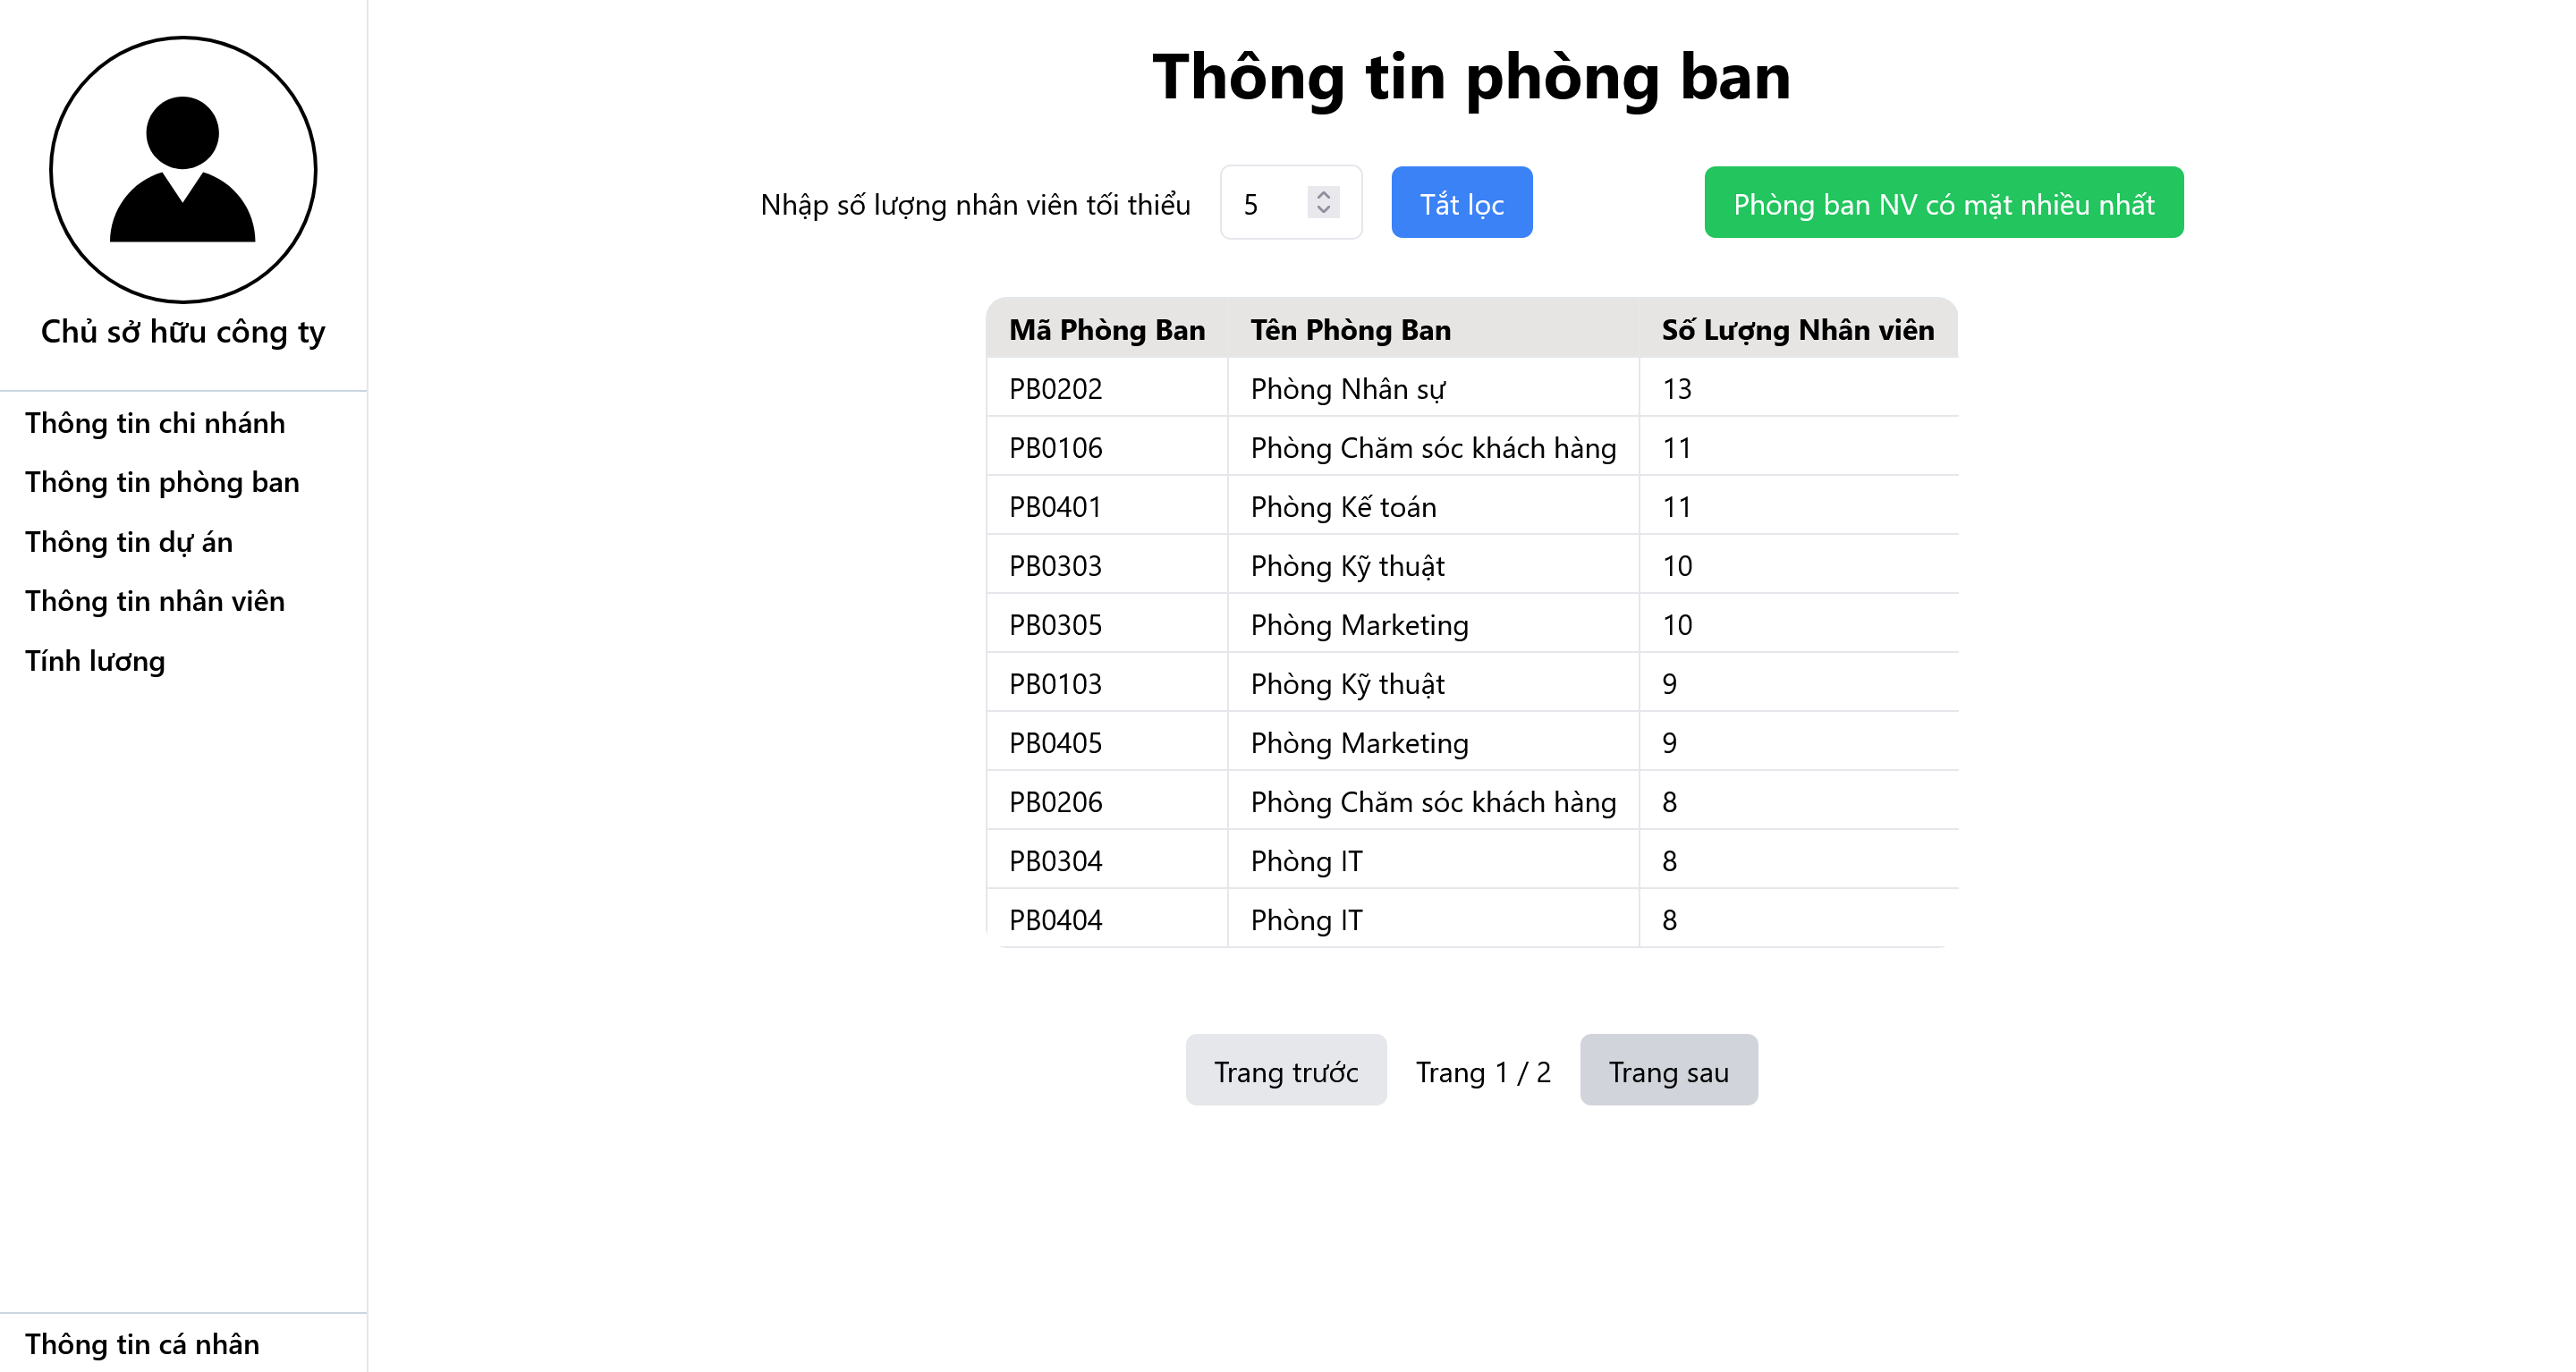
\includegraphics[width=1\linewidth]{content/images/ManHinh_2_b.png}
    \caption{Màn hình lọc phòng ban có số lượng nhân viên lớn hơn 5}
    \label{fig:ManHinh_2_b}
\end{figure}

Để sử dụng tính năng sắp xếp các phòng ban theo thứ tự giảm dần tổng số ngày có mặt của các nhân viên, người dùng nhấn vào nút 'Phòng ban NV có mặt nhiều nhất'. Để quay lại bảng thông tin phòng ban bình thường sau khi sử dụng tính năng, người dùng click vào nút 'Tắt hiển thị'.
\begin{figure}[H]
    \centering
    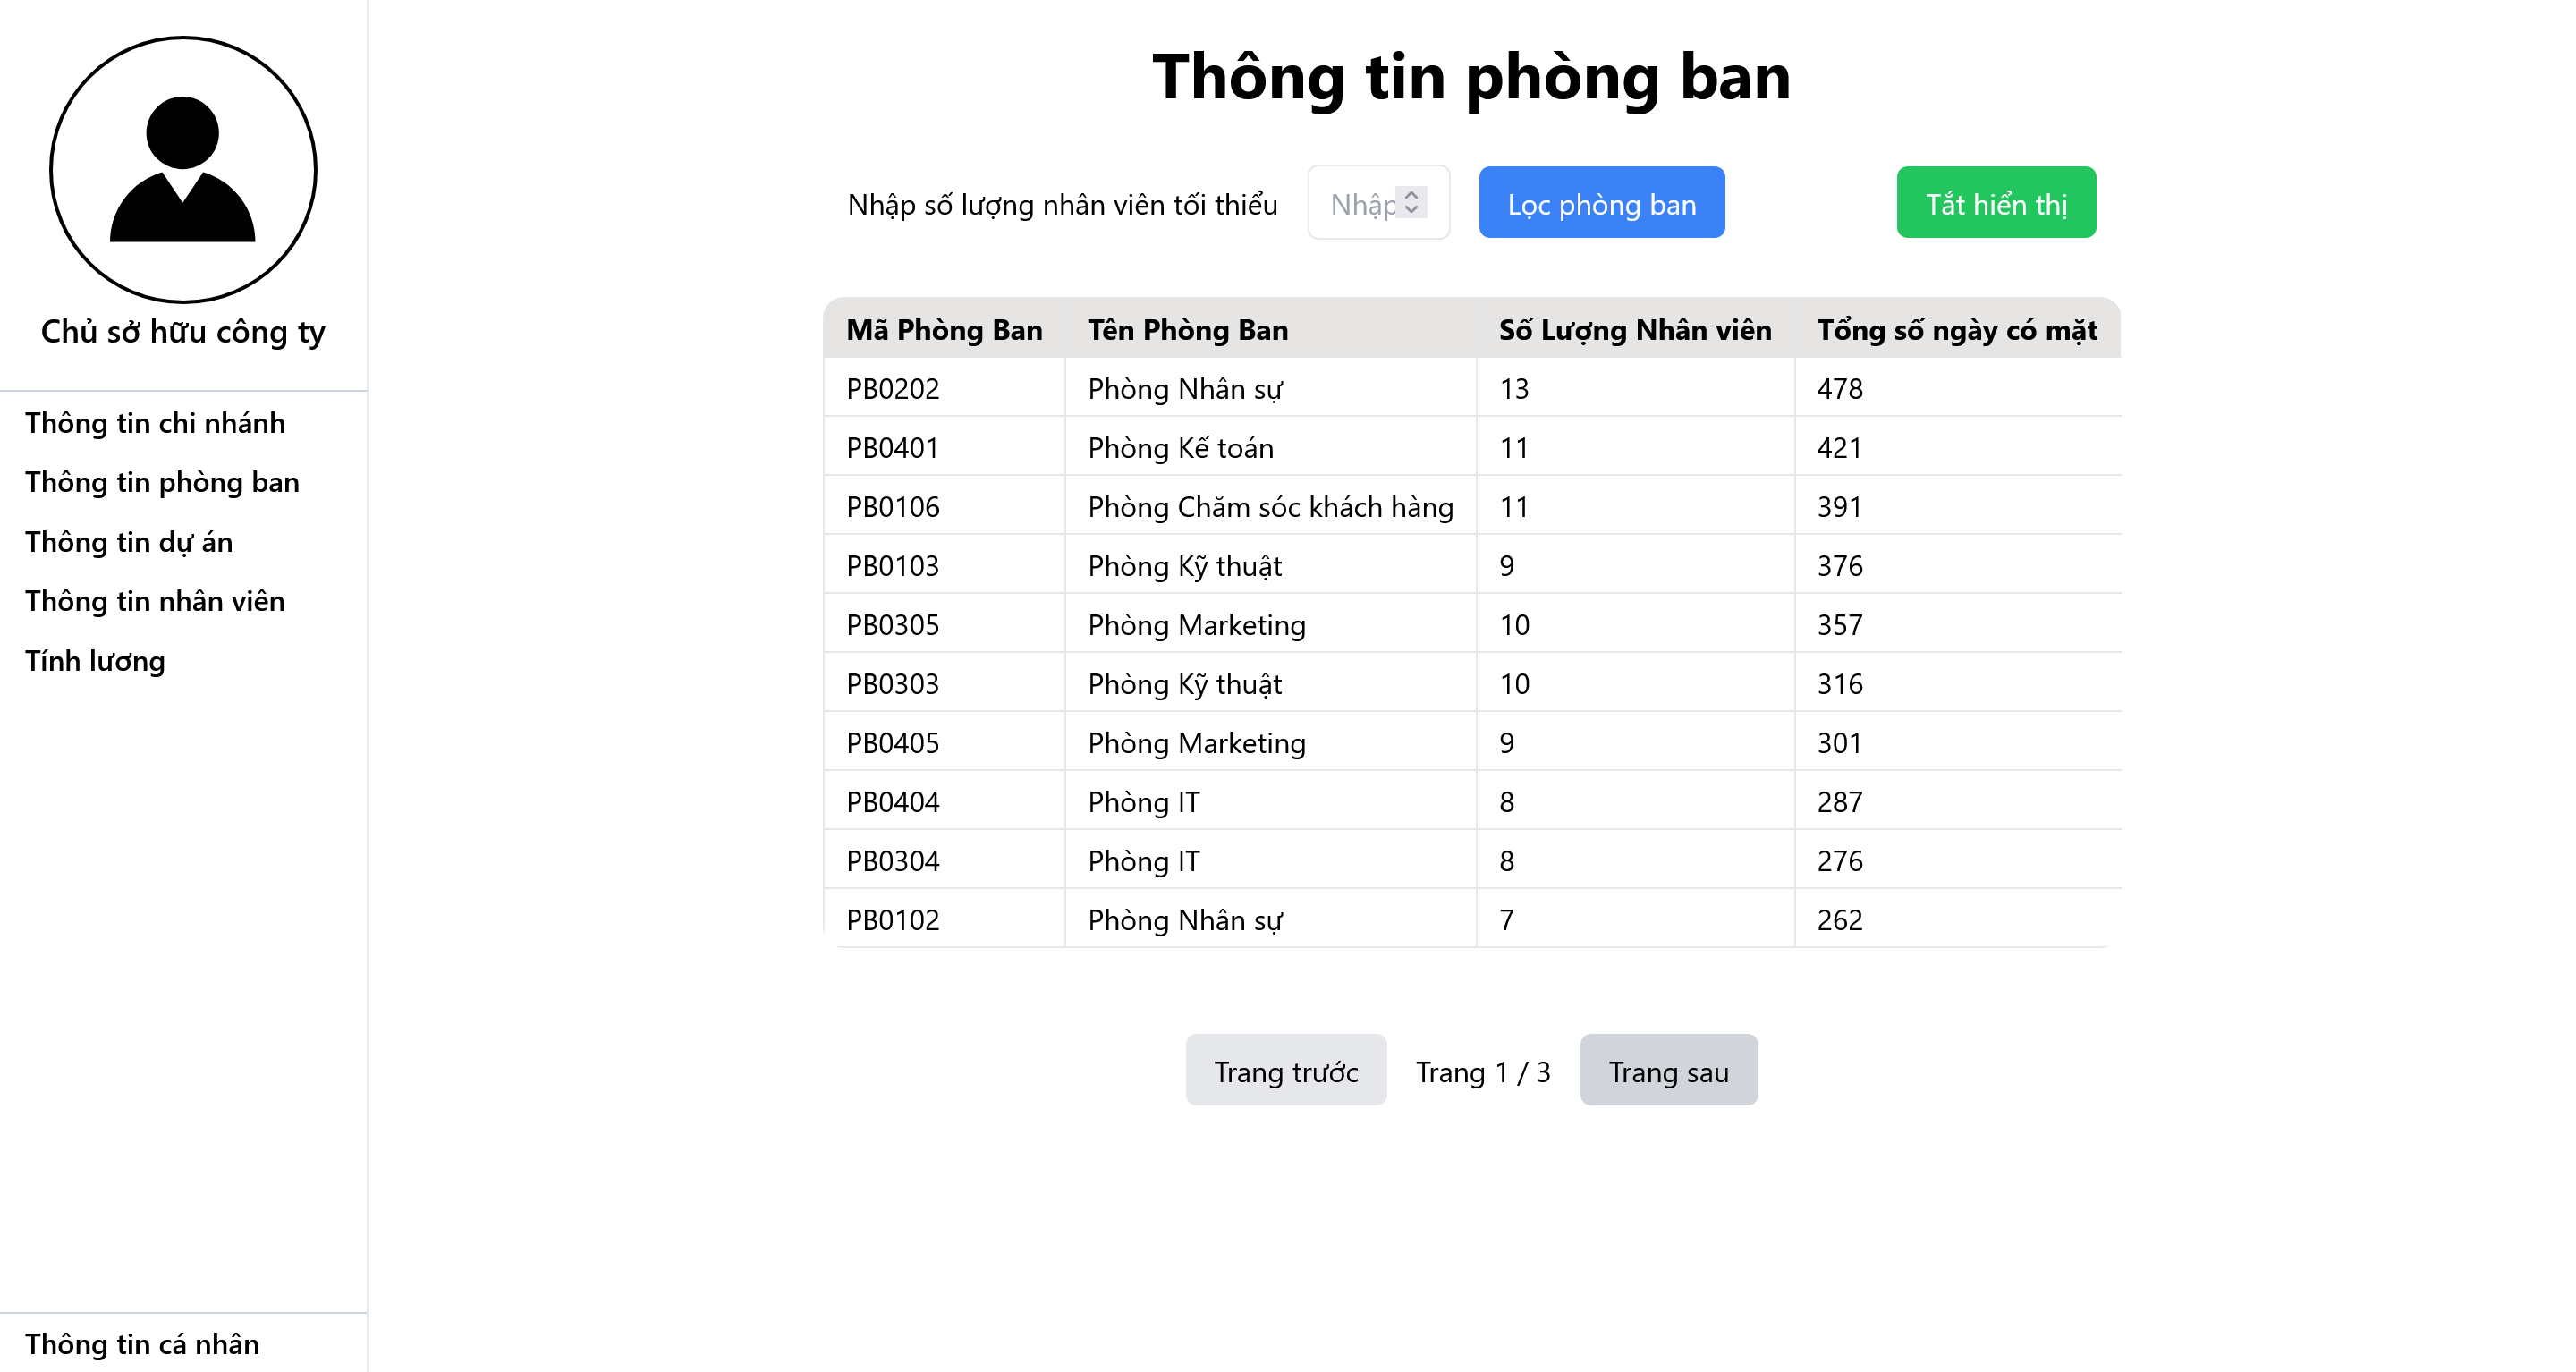
\includegraphics[width=1\linewidth]{content/images/ManHinh_2_c.png}
    \caption{Màn hình sắp xếp phòng ban dựa trên số ngày có mặt của nhân viên}
    \label{fig:ManHinh_2_c}
\end{figure}

\newpage
Để hiện thực màn hình trên, chúng em tạo 3 components tượng trưng cho 3 bảng với số cột khác nhau, mỗi bảng tương ứng với một trong các chức năng sau:
\begin{itemize}
    \item [--] Xem thông tin phòng ban và nhân viên vận hành.
    \item [--] Xem thông tin các phòng ban có số nhân viên lớn hơn một con số cụ thể.
    \item [--] Hiển thị phòng ban theo thứ tự giảm dần số ngày có mặt của nhân viên.
\end{itemize}
\begin{minted}{jsx}
    // Component để hiển thị bảng thông tin phòng ban và nhân viên vận hành.
    function PhongBanTable(props) {
        const headers = ['Mã Phòng Ban', 'Tên Phòng Ban', 'Mã Chi Nhánh', 'Số Lượng Nhân viên', 'MSNV Vận Hành', 'Tên NV vận hành', /*'MSNV Quản Lý', 'Tên NV quản lý',*/ "Tùy chỉnh"]

        return (
            <Table columnHeaders={headers} rowsData={props.rowsData}/>
        )
    }
    // Component để hiển thị bảng xem thông tin phòng ban có số nhân viên lớn hơn một con số cụ thể.
    function PhongBanTable2({ rowsData }) {
        const headers = ['Mã Phòng Ban', 'Tên Phòng Ban', 'Số Lượng Nhân viên'];

        return (
            <Table columnHeaders={headers} rowsData={rowsData} />
        );
    }
    // Component để hiển thị phòng ban theo thứ tự giảm dần số ngày có mặt của nhân viên.
    function PhongBanTable3({ rowsData }) {
        const headers = ['Mã Phòng Ban', 'Tên Phòng Ban', 'Số Lượng Nhân viên', 'Tổng số ngày có mặt'];

        return (
            <Table columnHeaders={headers} rowsData={rowsData} />
        );
    }

    // Việc bảng nào sẽ được hiển thị được xác định bởi trạng thái của hai biến showMaxPresence và filterEnabled
    {showMaxPresence ? (
        <PhongBanTable3 rowsData={currentRows} />
    ) : filterEnabled ? (
        <PhongBanTable2 rowsData={currentRows} />
    ) : (
        <PhongBanTable rowsData={currentRows} />
    )}
\end{minted}

\newpage
Câu lệnh gọi API và render dữ liệu cho bảng thông tin phòng ban và nhân viên vận hành.
\begin{minted}{jsx}
    // BACK-END
    // API để lấy thông tin về phòng ban cùng nhân viên vận hành phòng ban đó
    export const getPhongBanInfo_Manager = async () => {
        const rows = await ReadQuery(`SELECT nhanvien.\`MaPhongBan\`, \`TenPhongBan\`, \`MaChiNhanh\`, \`SoLuongNhanVien\`, nhanvien.\`MaNV\`, CONCAT (nhanvien.\`Ho\`,' ', nhanvien.\`TenLot\`,' ', nhanvien.\`Ten\`) as 'TenVanHanh' from phongban JOIN nhanvien ON phongban.\`MSNV_VanHanh\`=nhanvien.\`MaNV\`;`)
        return rows;
    }
    app.get('/api/phongban', async function (req, res) {
        const phongbaninfo = await getPhongBanInfo_Manager();
        res.send({phongbaninfo})
    })

    // FRONT-END
    // Gọi API để lấy thông tin 
    const fetchPhongBan = async () => {
        try {
            const res = await fetch("/api/phongban");
            const data = await res.json();
            console.log(data);
            setPhongBan(data.phongbaninfo);
        } catch (error) {
            console.log(error);
        }
    };
    // Các câu lệnh phục vụ việc phân trang
    // Xác định dữ liệu cho trang hiện tại
    const totalPages = Math.ceil(phongBan.length / rowsPerPage);
    // currentRows sẽ chứa thông tin của phòng ban và nhân viên vận hành tại trang currentPage
    const currentRows = phongBan.slice(
        (currentPage - 1) * rowsPerPage,
        currentPage * rowsPerPage
    );
    // Truyền dữ liệu cho component PhongBanTable để render bảng dữ liệu
    <PhongBanTable rowsData={currentRows} />
\end{minted}

\newpage
Câu lệnh gọi API và render dữ liệu cho bảng các phòng ban có số nhân viên lớn hơn một con số cụ thể.
\begin{minted}{jsx}
    // BACK-END
    // API để lấy thông tin về các phòng ban có số nhân viên lớn hơn một con số cụ thể.
    export const getPhongBanCoSoLuongNhanVienLonHon = async (min) => {
        const rows = await ReadFromProcedureQuery(`CALL LocPhongBanCoSoLuongNhanVienLonHon(${min})`);
        return rows;
    };
    app.get('/api/phongban-co-nhanvien-lon-hon', async (req, res) => {
        const { min } = req.query; // Lấy tham số "min" từ query string
        if (!min) {
            return res.status(400).json({
                success: false,
                message: 'Vui lòng cung cấp tham số "min"',
            });
        }

        try {
            const filteredPhongBan = await getPhongBanCoSoLuongNhanVienLonHon(min);
            res.status(200).json({
                success: true,
                filteredPhongBan,
            });
        } catch (error) {
            console.error(error);
            res.status(500).json({
                success: false,
                message: 'Lỗi server',
            });
        }
    });
\end{minted}
\begin{minted}{jsx}
    // FRONT-END
    // Input field để người dùng nhập số lượng nhân viên tối thiểu
    <input
        type="number"
        placeholder="Nhập số lượng nhân viên tối thiểu"
        value={filterValue}
        onChange={(e) => setFilterValue(e.target.value)}
    />
    // Khi người dùng nhấn nút 'Lọc phòng ban', hàm fetchFilteredPhongBan sẽ được gọi để lấy thông tin 
    const fetchFilteredPhongBan = async () => {
        try {
            const res = await fetch(`/api/phongban-co-nhanvien-lon-hon?min=${filterValue}`);
            const data = await res.json();
            if (data.success) {
                setPhongBan(data.filteredPhongBan);
            } else {
                console.error("Không có dữ liệu sau khi lọc.");
            }
        } catch (error) {
            console.error("Lỗi khi lọc dữ liệu:", error);
        }
    };
    // Các câu lệnh phục vụ việc phân trang
    // Dữ liệu của trang currentPage lúc này được lưu ở thực thể currentRows
    // Truyền dữ liệu cho component PhongBanTable để render bảng dữ liệu
    <PhongBanTable2 rowsData={currentRows} />
\end{minted}

\newpage
Câu lệnh gọi API và render dữ liệu cho bảng hiển thị phòng ban theo thứ tự giảm dần số ngày có mặt của nhân viên.
\begin{minted}{jsx}
    // BACK-END
    // API để lấy dữ liệu phòng ban theo thứ tự giảm dần số ngày có mặt của nhân viên.
    export const getPhongBanCoSoLuongNhanVienCoMatNhieuNhat = async () => {
        try {
            const rows = await ReadFromProcedureQuery('CALL LocPhongBanCoSoLuongNhanVienCoMatNhieuNhat');
            return rows;
        } catch (error) {
            console.error(error);
            throw error;  // Rerun the error if needed for logging
        }
    };
    app.get('/api/phongban-nhanvien-comatnhieunhat', async (req, res) => {
        try {
            const maxPresencePhongBan = await getPhongBanCoSoLuongNhanVienCoMatNhieuNhat();  // Hàm này sẽ gọi thủ tục bạn đã tạo
            res.status(200).json({
                success: true,
                maxPresencePhongBan,
            });
        } catch (error) {
            console.error(error);
            res.status(500).json({ 
                success: false, 
                message: 'Lỗi khi lấy dữ liệu phòng ban' 
            });
        }
    });
\end{minted}
\begin{minted}{jsx}
    // FRONT-END
    // Khi nhấn nút 'Phòng ban NV có mặt nhiều nhất', hàm sau sẽ được gọi để gọi API trên
    const fetchMaxPresencePhongBan = async () => {
        try {
            const res = await fetch("/api/phongban-nhanvien-comatnhieunhat");
            const data = await res.json();
            if (data.success) {
                setPhongBan(data.maxPresencePhongBan);
            } else {
                console.error("Không có dữ liệu phòng ban có mặt nhiều nhất.");
            }
        } catch (error) {
            console.error("Lỗi khi fetch dữ liệu phòng ban có mặt nhiều nhất:", error);
        }
    };

    // Các câu lệnh phục vụ việc phân trang
    // Dữ liệu của trang currentPage lúc này được lưu ở thực thể currentRows
    // Dữ liệu được truyền xuống component hiển thị phòng ban theo thứ tự giảm dần số ngày có mặt của nhân viên để render bảng thông tin.
    <PhongBanTable3 rowsData={currentRows}
\end{minted}

\newpage